\subsection{Physical reach and an executed segmentation comparison}
Proseg 3.2.0 completed on both lung crops after disabling factorization following a default-run failure on the first small crop. It retained 5,774 and 1,482 transcripts, excluding 73 and 41. We compare counts on shared retained IDs at the original observed coordinates; Proseg's diffused coordinates define a different observation problem. These same-donor, sparse-crop runs provide alternative counts, rather than ownership truth.

A post-review protocol fixed three width settings before rerunning geometry-only extraction. The largest band-implied displacement caps among accepted patches are $0.451$, $1.352$ and $3.155\,\mu\mathrm m$. The enlarged halfwidth is accepted in 132 of 544 intermediate-cap patches and 41 of 543 largest-cap patches; the others retain halfwidth at most 4. At unlimited area, reachable changed nuclear counts are $186/1{,}134$, $223/1{,}134$ and $190/1{,}134$; Proseg counts are $185/2{,}798$, $241/2{,}798$ and $200/2{,}798$ (Fig.~\ref{fig:reach}). Exact score-spectrum membership is tested, including gaps between attainable counts. Excluded molecules remain zero-score geometric constraints. This refines the original nuclear protocol by retaining six additional boundary-gene questions, one reachable. Greedy reconstruction and different fallback ladders produce non-nested families, explaining why reach can decrease at the largest cap. Even the best tested setting reaches only $19.7\%$ of changed nuclear counts and $8.6\%$ of changed Proseg counts. Width and area increases therefore leave substantial restrictions from fixed seams, candidate neighbors and nuclear constraints.

\begin{figure}[ht]
\centering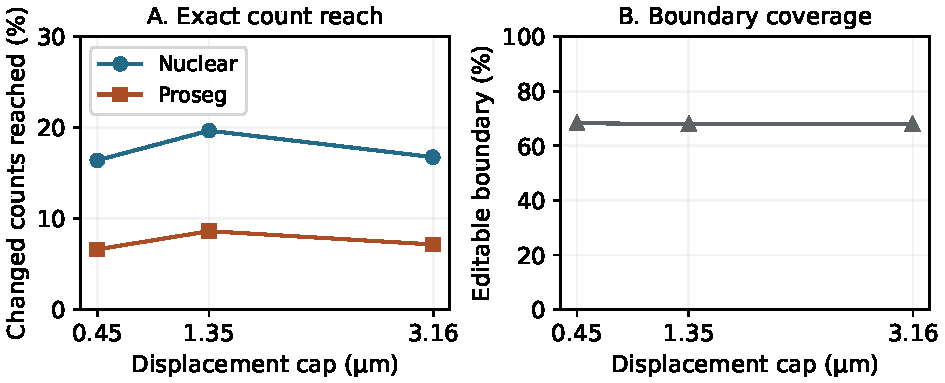
\includegraphics[width=.96\textwidth]{figures/reach_width.pdf}
\caption{Lung width sensitivity on fixed comparison populations. Left: exact countwise reach at unlimited area. Right: editable fraction of eligible-cell incident boundary edges. The rebuilt atlases are non-nested; connecting lines organize the tested settings. Reach describes each count separately, rather than joint feasibility or biological accuracy.}
\label{fig:reach}
\end{figure}
